\documentclass[a4paper]{article}

\usepackage{amsmath}
\usepackage{amssymb}
\usepackage{stellar}
\usepackage{parskip}
\usepackage{fullpage}
\usepackage{wrapfig}
\usepackage{tikz}
\usepackage{graphicx}

\usetikzlibrary{cd}

\title{Algebra lineare I}
\author{Paolo Bettelini}
\date{}

\begin{document}

\maketitle
\tableofcontents

\section{Algebra lineare}

La moltiplicazione scalare di un vettore è un \emph{omotetia}.

\sdefinition{Spazio a prodotto interno}{
    Uno \emph{spazio a prodotto interno} è uno spazio vettoriale con la struttura
    aggiuntiva del dot product.
}

\sdefinition{Ortogonalità}{
    In uno spazio a prodotto interno, la nozione di \emph{ortogonalità}
    è definita dalla nullità del product.
}

\sdefinition{Spazio affine}{
    Uno \emph{spazio affine} è uno spazio vettoriale
    senza la nozione del punto di origine.
}

Il prodotto vettoriale in \(\mathbb{R}^3\) necessita di un orientamento.
Se consideriamo il prodotto vettoriale di \(\mathbb{R}^3\)
nei piano bidimensionale \(\mathbb{R}^2\), il prodotto ha forma
di complesso. Il prodotto scalare e il prodotto dei complessi
si uniscono nella struttura quaternionale.

I sistemi lineari possono essere interpretati come trovare l'intersezione delle varie rette,
oppure possiamo vederlo come trovare i coefficienti lineari tali che la combinazione lineare
(con tali coefficienti) dei vettori sia il vettore risultante.
Possiamo quindi anche vederlo come trovare il vettore che moltiplicato dalla matrice del sistema
ci restituisce il vettore voluto.

\section{Algoritmo di eliminazione di Gauss}

\slemma{}{
    Dato un sistema di equazioni con \(m\) equazioni e \(n\) indeterminata,
    l'eliminazione di Gauss non modifica le soluzioni del sistema.
}

\sproof{}{
    Per la prima operazione, la dimostrazione in una direzione è banale.
    Per dimostrarla nell'altra direzione è sufficiente considerare le righe della matrice
    \(E_i' = E_i + \lambda E_j\) dove l'apice indica la riga modificata. Siccome la riga che viene aggiunta
    rimane invariata \(E_j = E_j'\) allora \(E_i = E_i' - \lambda E_j'\) e quindi
    i calcoli nella direzione inversa sono gli stessi in quanto sto sempre aggiungendo un multiplo di un'altra riga.
    Quindi le soluzioni prima e dopo l'operazione rimangono invariate. Se il sistema originario non ha soluzioni,
    non ne ha nemmeno quello nuovo.
}

Nell'eliminazionne di gauss vogliamo raggiungere la matrice triangolare superiore.
Distinguiamo i casi dove ci sono righe con tutti zero includendo o senza includere il termine noto.
In tali casi abbiamo infiniti o finite soluzioni.
Nel caso non sia possibile raggiungere la row echelon form, bisogna studiare i termini noti.

L'operazione della moltiplicazione scalare di una matrice ne modifica il determinante.
Usando solo le altre due operazioni non è quindi facile giungere alla reduced row echelon form.

Le matrici elementari \(E_{i,j}(\lambda)\) sono triangolari alte se \(i<j\) e basse \(i<j\).
Il valore non deve essere sulla diagonale.
Ripetere tale matrice \(E_1E_2E_3 \cdots A = U\) è come moltiplicare \(A\) per una singola matrice
(se non servono swap è triangolare inferiore). Se raggiunge la fine dell'eliminazione di gauss il risultato \(U\)
è triangolare superiore.
Il prodotto delle elementari è sostanzialmente le loro sovrapposizioni.

\sexercise{}{
    Dimostrare che il prodotto di matrici superiori o inferiori è superiore o inferiore.
}

\sexercise{}{
    Se \(A\) è invertibile, l'inverso è unico.
}

\sexercise{}{
    Le matrixi elementari sono invertibili e l'inversa di \(E_{i,j}(\lambda)\) è \(E_{i,j}(-\lambda)\)
}

\sexercise{}{
    Se \(A, B \in M_n(\mathbb{F})\) sono invertibili, allora \(AB\) e \(BA\)
    sono invertibili.
}

Siccome in \(E_1E_2E_3 \cdots A = U\) il prodotto delle elementari è invertibili, possiamo portarlo a destra.
Tale inversa è una matrice triangolare bassa. Abbiamo così dimostrato il

\stheorem{Fattorizzazione LU}{
    Sia \(Ax = B\) un sistema lineare non singolare dove non servono scambi.
    Allora il sistema è equivalente a
    \[
        LUx = B
    \]
    dove \(L\) è una matrice triangolare bassa con tutti \(1\) sulla diagonale principalmente,
    mentre \(U\) è una matrice triangolare alta con tutti i pivot sulla diagonale principale.
}

La fattorizazzione \(A=LU\) permette di trasformare la soluzione di un sistema
non singolare quadrato nelle soluzioni di due sistemi triangolari.
Sia \(y \triangleq Ux\). Allora dobbiamo risolvere
\(Ly = b\) che è un sistema triangolare inferiore nelle indeterminate \(y\),
e poi \(Ux = y\) che è un sistema triangolare superiore nelle indeterminate \(x\).
Se otteniamo \(LU\) allora il resto è banale.

Per eseguire gli scambi di righe possiamo costruire una matrice che è come la matrice
identità ma le righe dell'identità sono scambiate.
Questa è detta matrice di permutazione elementare \(P_{i,j}\).
Tale matrice è invertibile e la sua inversa è sè stessa.

Quindi l'eliminazione di Gauss usa \(E_{i,j}(\lambda)\) e \(P_{i,j}\).

\subsection{Algoritmi di Gauß-Jordan}

Dopo aver ridotto la matrice a scalini, è possibile usare una versione dell'algoritmo di
Gauss in senso inverso, cioè dal basso verso l'alto,
per ottenere una matrice che in ogni colonna contenente un pivot abbia solo il pivot come
numero non nullo, (questa matrice risultante è anche detta matrice a scalini in forma ridotta):
basta usare ogni riga, partendo dall'ultima, per eliminare tutte le
cifre diverse da zero che stanno sopra al pivot di questa riga.
Infine, sempre con mosse di Gauss (moltiplicando righe),
si può ottenere che ogni pivot abbia valore 1.

... Sia \(\hat{E}DE\) è l'inversa di \(A\). Se eseguo \(\hat{E}DE\) sull'identità ottengo
\[
    \hat{E}DEI_n = \hat{E}DE = A^{-1}
\]
sto quindi trasformando l'identità nell'inversa di \(A\).
Questa osservazione dà un metodo per il calcolo dell'inversa di una matrice non singolare
(Metodo di Gauss-Jordan)

\stheorem{}{
    Una matrice quadrata è non singolare se e solo se è invertibile.
}

\sproof{}{
    \iffproof{
        Se non è singolare, è invertibile per l'algoritmo di Gauß-Jordan.
    }{
        \(A\) invertibile, allora non esiste \(A^{-1}\) tale che \(A^{-1}A = I_n\).
        Sappiamo \(Ax = b\) implica \(A^{-1}(Ax) = A^{-1}b\) e quindi \(x = A^{-1}b\)
        è l'unica soluzione di \(Ax=b\), e quindi \(A\) è singolare.
    }
}

\section{Spazi vettoriali}

L'insieme vuoto non è uno spazio per nessun campo (manca l'esistenza).
Tuttavia, \(V = \{0\}\) può essere uno spazio vettoriale su ogni campo \(F\).

\sproposition{}{
    Let \(A\neq\emptyset\) be a set and let \(\mathbb{F}\) be a field.
    Consider the set
    \[
        {\mathbb{F}}^A \triangleq \{f\colon A \to \mathbb{F} \,|\, f \text{ is a function}\}
    \]
    Consider the operations
    \[
        +\colon {\mathbb{F}}^A \times {\mathbb{F}}^A \to {\mathbb{F}}^A
    \]
    given by \((f+g)(a) = f(a) + g(a)\)
    and the operation
    \[
        \cdot \colon \mathbb{F} \times {\mathbb{F}}^A \to {\mathbb{F}}^A
    \]
    given by \((f\cdot g)(a) = f(a)\cdot g(a)\).
    Then, \((\mathbb{F}, \mathbb{F}^A, +, \cdot)\) is a vector space.
}

In uno spazio vettoriale l'identità additiva è unica, l'inverso additivo è unico.

\subsection{Sottospazi vettoriali}

Gli assi cartesiani, una retta passante per l'origine (altrimenti non è soddisfatto il criterio del vettore nullo).


Uno spazio vettoriale è finito dimensionale se esiste un insieme finito di generatori.

\[
    \text{span}\left(
        \left\{
            E_{i,j} \,|\, 1 \leq i \leq n \land 1 \leq j \leq m
        \right\}
    \right)
    = \text{Mat}_{n\times m}(\mathbb{F})
\]

Ogni sottoinsieme di insieme linearmente indipendente è linearmente indipendente.

\sproposition{}{
    \[
        \text{Sym}(n) \oplus \text{Skew}(n) = M_{n\times n}(\mathbb{F})
    \]
}

\sproof{}{
    % lezione 10 ci sono i disegnigni per n=3
    Notiamo che \(A + A^t\) è simmetrica
    e \(A - A^t\) è antisimmetrico.
    Quindi sommiamo le due
    \begin{align*}
        A = \frac{A + A^t}{2} + \frac{A-A^t}{2}
    \end{align*}
    Alternativamente possiamo dimostrare che
    \[
        \text{dim}(\text{Sym}(n) + \text{Skew}(n)) = n^2
    \]
    Abbiamo quindi
    \begin{align*}
        \text{dim}(\text{Sym}(n) + \text{Skew}(n))
        &= \text{dim}(\text{Sym}(n)) + \text{dim}(\text{Skew}(n))
        - \text{dim}(\text{Sym}(n) \cap \text{Skew}(n))
    \end{align*}
    ma l'intersezione delle antisimmetriche e quelle simmetriche è solo la matrice nulla. Quindi
    \begin{align*}
        \text{dim}(\text{Sym}(n) + \text{Skew}(n))
        &= \text{dim}(\text{Sym}(n)) + \text{dim}(\text{Skew}(n))
    \end{align*}
    Notiamo che \(E_{i,j} + E_{j,i} \in \text{Sym}(n)\)
    e \(E_{i,j} - E_{j,i} \in \text{Skew}(n)\).
    Consideriamo il seguente insieme di matrici
    \[
        \{
            E_{i,j} + E_{k,l} \in M_n(\mathbb{F}) \,|\, i=l \land j = k \land (i,j) \leq (l,k)
        \}
        \cup
        \{
            E_{i,i} \in M_n(\mathbb{F})
        \}
    \]
    che è una base delle matrici simmetriche, e
    \[
        \{ E_{i,j} - E_{k,l} \in M_n(\mathbb{F}) \,|\, i=l \land j = k \land (i,j) \leq (l,k) \}
    \]
    che è una base delle matrici antisimmetriche.
    Quindi, la dimensione delle simmetriche è
    \[
        \text{dim}(\text{Sym}(n)) = \sum_{i=1}^n i = \frac{n(n+1)}{2}
    \]
    mentre per quelle antisimmetriche la diagonale principale è vietata e quindi la dimensione è
    \[
        \text{dim}(\text{Skew}(n)) = \sum_{i=1}^{n-1} i = \frac{n(n-1)}{2}
    \]
    E infatti
    \[
        n^2 = \frac{n(n-1)}{2} +  \frac{n(n+1)}{2}
    \]
    e quindi siccome
    \[
        \text{Sym}(n) + \text{Skew}(n) = M_{n\times n}(\mathbb{F})
    \]
    e
    \[
        \text{Sym}(n) \cap \text{Skew}(n) = \{0\}
    \]
    abbiamo che
    \[
        \text{Sym}(n) \oplus \text{Skew}(n) = M_{n\times n}(\mathbb{F})
    \]
}

Vogliamo dimostrare ora che \(\text{dim}_{\mathbb{Q}}(\mathbb{R}) = \infty\).
Consideriamo l'insieme
\[
    \{
        \ln p_1, \ln p_2, \cdots, \ln p_n    
    \}
\]
di logaritmi di primi. Tale insieme è linearmente indipendente su \(\mathbb{Q}\)
ed è arbitrariamente largo.
Dobbiamo anche dimostrare che \(\ln p_1\) è irrazionale (tra l'altro di tutti gli interi non solo dei primi).
Per mostrarlo abbiamo
\[
    0 = \sum \alpha_i v_i
\]
dove \(\alpha_i \in \mathbb{Q}\).
Moltiplicando per il massimo denominatore degli \(\alpha_i\)
trasformiamo i coefficienti in \(\mathbb{Z}\)
\begin{align*}
    0 &= \sum n_i \ln p_i \\
    1 &= \text{exp}\left\{
        \sum n_i \ln p_i
    \right\} \\
    &= \text{exp}\left\{
        \sum \ln p_i^{n_i}
    \right\} \\
    &= e^0
\end{align*}
ma quindi
\[
    1 = \prod p_i^{n_i} \iff n_i = 0
\]
che è nullo per il teorema fondamentale dell'aritmetica.
Quindi non esiste nessuna collezione finita che genera.

\pagebreak

\section{Spazi affini}

% se (p0, p1, ..., pn) sono affinamente indipendenti
% allora anche (p1, p0, ... pn) etc. lo sono
% c'è un azione del gruppo simmetrico su tali vettori

\section{Altro}

Spazi vettoriali e moduli visti come azioni di gruppi abeliani

Lo spazio delle trasformazioni lineari \(\mathcal{L}(V, W)\) è un sottospazio vettoriale
di \(W^V\). Inoltre, \((\text{Env}(V), +, \circ)\) è un anello
e \((\text{Env}(V), +, \circ, \cdot)\) è una \(\mathbb{F}\)-algebra non necessariamente commutativa.
Una trasformazione è iniettiva se e solo se \(\ker f = \{0\}\).
Anche l'immagine di \(f \in \mathcal{L}(V, W)\) è un sottospazio.

\section{Isomorfismi fra spazi vettoriali}

\sdefinition{Isomorfismi fra spazi vettoriali}{
    Fra \(V\) e \(W\) è un'applicazione lineare invertibile fra \(V\) e \(W\).
}

Dato uno spazio \(V\) finito dimensionale con base \(\mathcal{B} = \{v_1, \cdots, v_n\}\)
la mappa \(\Phi_\mathcal{B} \colon V \to \mathbb{F}^n\) che porta un vettore
alla sua tupla delle coordinate è un isomorfismo.
Infatti, il suo kernel sono i vettori che vanno nelle coordinate nulle.
Siccome la base è linearmente indipendente, l'ultimo tale vettore è quello nullo.
Quindi, contiene solo un elemento ed è quindi iniettivo.
Inoltre, dato un elemento \((a_1, \cdots, a_n)\), la preimmagine è \(v_1a_1 + \cdots + v_na_n\).
Ogni scelta di base fornisce un diverso isomorfismo.

\stheorem{}{
    Siano \(V, W\) due \(\mathbb{F}\)-spazi vettoriali finito dimensionali.
    Allora, \(V\) e \(W\) sono isomorfismi se e solo se hanno la stessa dimensione.
}

\sproof{}{
    \iffproof{
        Sia \(f\colon V \to W\) un isomorfismo. Allora \(f\) è invertibile quindi iniettiva e suriettiva.
        \[
            \text{dim} V = \text{dim ker} f + \text{dim Im} f = \text{dim} W
        \]
    }{
        Let \(n = \text{dim} V = \text{dim W}\). Sia \(\mathcal{B} = \{v_1, \cdots, v_n\}\)
        una base per \(V\) e \(\mathcal{L} = \{w_1, \cdots, w_n\}\) una base per \(W\). Abbiamo isomorfismi
        \(\Phi_\mathcal{B}\colon V \to \mathcal{F}^n\) e \(\Phi_\mathcal{L}\colon W \to \mathcal{F}^n\)
    }
    % https://tikzcd.yichuanshen.de/#N4Igdg9gJgpgziAXAbVABwnAlgFyxMJZABgBpiBdUkANwEMAbAVxiRADUQBfU9TXfIRQAmclVqMWbAOrdeIDNjwEiARlKrx9Zq0QgAOvoC2dHAAsARheAAxLgD1CXcTCgBzeEVAAzAE4QjJHUQHAgkUQkdNkMABTMsAH1gQxNzAGNGYAAZLi45H39AxAjQpDJIqT1Y+KSU0zMMhmAAIVz8kD8AsupSxGDtSoN9OMTk43rG7Nz7YABaVS4AAkM0rF805eGasdSGzNa8ngKu4p6wvuoLGDAoJFmAFgBOagY6K4YY-mUhEF8sNzMOBA1AGuiGI1q43SmRyDjmC24FC4QA
}
\begin{center}
    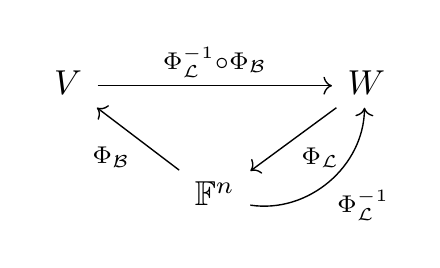
\begin{tikzpicture}
        \node[scale=1.25] {
            \begin{tikzcd}
                V \arrow[rr, "\Phi_{\mathcal{L}}^{-1} \circ \Phi_{\mathcal{B}}"] &                                                                                                     & W \arrow[ld, "\Phi_{\mathcal{L}}"] \\
                                                                                & \mathbb{F}^n \arrow[lu, "\Phi_{\mathcal{B}}"] \arrow[ru, "\Phi_{\mathcal{L}}^{-1}"', bend right=49] &                                   
                \end{tikzcd}
        };
        \end{tikzpicture}
\end{center}

\stheorem{}{
    Siano \(V, W\) spazi vettoriali \(n\) dimensionali su un campo \(\mathbb{F}\) e sia
    \(f \in \mathcal{L}(V, W)\). Sono equivalenti:
    \begin{enumerate}
        \item \(f\) è invertibile
        \item \(f\) è iniettiva
        \item \(f\) è suriettività
    \end{enumerate}
}

\sproof{}{
    \begin{itemize}
        \item \((1) \implies (2)\): se è invrtibile è anche iniettiva.
        \item \((2) \implies (3)\): siccome \(f\) è iniettiva, \(\text{ker} f\) è ridotto
        al vettore nullo. Abbiamo
        \[
            \text{dim Im} f = \text{dim} V - \text{dim ker} f
            = \text{dim} V = \text{dim} W
        \]
        Ma allora \(\text{Im} f = W\) e quindi è suriettiva.
        \item \((3) \implies (1)\): basta mostrare che \(f\) è iniettiva.
        \[
            \text{Im} f = W \implies \text{dim Im} f = \text{dim} W = \text{dim} V
        \]
        quindi
        \[
            \text{dim ker} f = \text{dim} V - \text{dim Im} f = 0
        \]
        il che implica che il kernel sia nullo e quindi \(f\) è iniettiva.
    \end{itemize}
}

\subsection{Sistemi lineari non quadrati}

\sproof{Rouché-Capelli}{
    \iffproof{
        Supponiamo che \(Ax = b\) abbia soluzione e mostriamo che il rango
        della matrice completa è pari al rango della matrice \(\text{rank} A|b = \text{rank} A\).
        Sia \(\overline{x} \in \mathbb{F}^n\) una soluzione di  \(Ax = b\).
        Allora \(A\overline{x} = b\) è equivalente a
        \[
            \sum_i \overline{x}_i A^i = b \iff b \in \text{span}(A^1, \cdots, A^n)
        \]
        but then
        \[
            \text{rank}(A|b) = \text{dim span}(A^1, \cdots, A^n, b) = \text{dim span}(A^1, \cdots, A^n)
            = \text{rank} A
        \]
    }{
        Supponiamo che i due ranghi siano uguali. Ma allora il sottospazio generato dalle colonne di \(A\)
        coincide con il sottospazio generato dalle colonne di \(A|b\). In particolare esistono scalari
        \(\overline{x}_i\) tali che
        \[
            b = \sum_i \overline{x}_i A^i \iff A\overline{x} = b
        \]
        Quindi \(ax = b\) ammette soluzioni.
        Sappiamo già che l'insieme delle soluzioni è un sottospazio affine di \(\mathbb{A}^n(\mathbb{F})\)
        diretto da \(\text{ker} A\). Osserviamo che
        \[
            \text{ker} A = \{x \in \mathbb{F}^n \,|\, Ax = 0\} = \text{ker} L_A
        \]
        dove \(L_A \colon \mathbb{F}^n \to \mathbb{F}^n\).
        \begin{align*}
            n = \text{dim} \mathbb{F}^n &= \text{dim ker} L_A + \text{dim Im} L_A
            = \text{dim ker} A + \text{rank} L_A \\
            &= \text{dim ker} A + \text{rank} A \implies \text{dim ker} A = n-\text{rank} A
        \end{align*}
    }
}

\sproposition{}{
    L'eliminazione di Gauss non varia il rango di una matrice
}

\end{document}